\documentclass[12pt,a4paper]{article}

% =========================
% Temel paket yüklemeleri
% =========================
\usepackage[utf8]{inputenc}
\usepackage[T1]{fontenc}
\usepackage[english]{babel}

% Sayfa yapısı ve kenar boşlukları
\usepackage[margin=2.5cm]{geometry}

% Satır aralığını 1.5 yapıyorum
\usepackage{setspace}
\onehalfspacing

% Matematik ortamları için gerekli paketler
\usepackage{amsmath, amssymb}

% Tablo paketleri
\usepackage{booktabs}
\usepackage{longtable}
\usepackage{array}
\usepackage{multicol}

% Görselleri kullanmak için
\usepackage{graphicx}
\usepackage{float}
\usepackage{caption}

% Linkleri düzenlemek için
\usepackage[hidelinks]{hyperref}

% Algoritma paketleri
\usepackage{algorithm}
\usepackage{algpseudocode}

% =========================
% Renk tanımları
% =========================
\usepackage{xcolor}
\definecolor{richmaroonxd}{RGB}{186, 52, 90}

% =========================
% Algoritma anahtar kelimelerinin renk ve yazım stilini ayarlıyorum
% =========================
\algrenewcommand\algorithmicprocedure{\textbf{\textcolor{richmaroonxd}{Procedure}}}
\algrenewcommand\algorithmicwhile{\textbf{\textcolor{richmaroonxd}{While}}}
\algrenewcommand\algorithmicfor{\textbf{\textcolor{richmaroonxd}{For}}}
\algrenewcommand\algorithmicforall{\textbf{\textcolor{richmaroonxd}{For all}}}
\algrenewcommand\algorithmicif{\textbf{\textcolor{richmaroonxd}{If}}}
\algrenewcommand\algorithmicelse{\textbf{\textcolor{richmaroonxd}{Else}}}
\algrenewcommand\algorithmicreturn{\textbf{\textcolor{richmaroonxd}{Return}}}
\algrenewcommand\algorithmicend{\textbf{\textcolor{richmaroonxd}{End}}}

% Algoritma input-output başlıkları
\algnewcommand\algorithmicinput{\textbf{\textcolor{richmaroonxd}{Input:}}}
\algnewcommand\Input{\item[\algorithmicinput]}
\algnewcommand\algorithmicoutput{\textbf{\textcolor{richmaroonxd}{Output:}}}
\algnewcommand\Output{\item[\algorithmicoutput]}

% Fonksiyon isimleri için ufak bir kolaylık
\newcommand{\Func}[1]{\textcolor{richmaroonxd}{#1}}
\usepackage{listings}
\usepackage{xcolor}

% Atom One Light renkleri
\definecolor{atom-bg}{HTML}{FAFAFA}
\definecolor{atom-blue}{HTML}{007ACC}
\definecolor{atom-purple}{HTML}{AF00DB}
\definecolor{atom-green}{HTML}{098658}
\definecolor{atom-gray}{HTML}{6A6A6A}
\definecolor{atom-orange}{HTML}{D16969}

\lstdefinestyle{atomone}{
    backgroundcolor=\color{atom-bg},
    basicstyle=\ttfamily\small,
    keywordstyle=\color{atom-blue}\bfseries,
    stringstyle=\color{atom-green},
    commentstyle=\color{atom-gray}\itshape,
    numberstyle=\tiny\color{atom-gray},
    numbers=left,
    stepnumber=1,
    numbersep=10pt,
    frame=single,
    rulecolor=\color{atom-gray},
    tabsize=4,
    showstringspaces=false,
    breaklines=true,
    emph={
        True, False, None,
        int, float, str, list, dict, set, tuple,
        range, len, print, return
    },
    emphstyle=\color{atom-purple}\bfseries,
    moredelim=**[is][\color{atom-orange}]{@}{@}  % özel vurgular için
}

% Kolay kullanım komutu
\newcommand{\pythoncode}[2]{
\begin{lstlisting}[style=atomone,caption={#1}]
#2
\end{lstlisting}
}
\usepackage{tikz}
\usepackage[table]{xcolor}
\usepackage{pgfplots}
\pgfplotsset{compat=1.18}

% =========================
% Bölüm numaralandırma stilini ayarlıyorum
% =========================
\renewcommand{\thesection}{\arabic{section}}
\renewcommand{\thesubsection}{\arabic{section}.\arabic{subsection}}

% =========================
% Başlık bilgileri
% =========================
\title{\textbf{Solving the U-shaped Assembly Line Balancing Problem Type-II\\Using a Genetic Algorithm}}

\author{
Firuze İpek Yıldırım \quad 2220469028 \\
Mustafa Alp Ulaş \quad 2210469034 \\
Beril Yıldız \quad 2230469107 \\
Pınar Ece Pank \quad 2240469085 \\
Tarık Buğra Birinci \quad 2210469046 \\[6pt]
\textit{Department of Industrial Engineering, Hacettepe University}
}

\date{Project Final Report\\December 2025}

% =========================
% DOKÜMAN BAŞLANGICI
% =========================
\begin{document}


% KAPAK SAYFASI

\begin{titlepage}
    \centering
    \vspace*{2cm}

    {\LARGE \textbf{Solving the U-Shaped Assembly Line Balancing Problem Type-II \\[2mm]
    Using a Genetic Algorithm}} \par

    \vspace{1.4cm}

    {\large \textbf{Project Final Report}} \\[0.4cm]
    {\large EMU427 -- Heuristic Methods for Optimization} \\[0.3cm]
    {\large Department of Industrial Engineering \\ Hacettepe University}

    \vspace{2cm}

    {\large \textbf{Students}} \\[0.5cm]

    \begin{center}
        \begin{tabular}{l r}
            Firuze İpek Yıldırım & 2220469028 \\
            Mustafa Alp Ulaş     & 2210469034 \\
            Beril Yıldız         & 2230469107 \\
            Pınar Ece Pank       & 2240469085 \\
            Tarık Buğra Birinci  & 2210469046 \\
        \end{tabular}
    \end{center}

    \vspace{1.6cm}

    {\large \textbf{Instructor:} Prof. Çağrı Koç}

    \vfill
    {\large December 2025 \\ Ankara, Türkiye}
\end{titlepage}


% İÇİNDEKİLER

\tableofcontents
\newpage


% INTRODUCTION

\newpage
\section{Introduction}
% Bu bölümde: U-shaped assembly line kavramı, literatür özeti,
%%%%%%%%%%% !!!!!!!!!!!!!!documentten copy paste yap ipek
% UALBP-II’nin neden önemli olduğu ve GA seçme motivasyonumuz anlatılacak.
Assembly line balancing is one of the major problems in industrial engineering that it
produces the optimal division of the worker tasks to maximize the output and minimize
the idle time. Present-day manufacturing is characterized by the demand for lower prices,
greater flexibility, and shorter production times, thus making good line balancing absolutely
necessary. Although traditional straight lines have been in use for a long time, U-shaped
assembly lines have been very much favored because they allow workers to work on both
sides of the line, thus cutting down on the traveling time and making multi-tasking easier.
Here we consider the U-shaped Assembly Line Balancing Problem Type-II (UALBP-2).
Contrasting with Type-I problems that minimize the number of stations for a given cycle
time, UALBP-2 seeks to minimize the cycle time for a fixed number of workstations. This
formulation is especially suitable for plants with fixed physical layouts where the production
rate is to be maximized.
The UALBP-2 is an NP-hard combinatorial problem, meaning that as the number of
tasks increases, the exact optimization methods become computationally impractical. The
flexibility of U-lines, which allows tasks to be assigned from either the front (forward) or
the back (reverse) of the precedence graph, significantly expands the search space. This
complexity is addressed in this project by a Genetic Algorithm (GA) implementation. GAs
are stochastic search methods inspired by natural evolution, capable of exploring the global
solution space and avoiding local optima through mechanisms like crossover and mutation.
The report is organized as follows: Section 2 provides the mathematical formulation of the
UALBP-2 and describes the dataset ARC83 used in this study. Section 3 details the proposed
Genetic Algorithm, including chromosome representation and genetic operators. Section 4
presents the computational results, followed by the contribution to Sustainable Development
Goals in Section 5 and the conclusions in Section 6.

% PROBLEM FORMULATION

\newpage
\section{Problem Formulation}

\subsection{UALBP-II Definition}
% Burada problemi resmi olarak tanımlayacağım: amaç fonksiyonu, cycle time,
% sabit istasyon sayısı ve U-shaped yapıdaki yön değişimleri.
The Type 2 U-shaped Assembly Line Balancing Problem (UALBP-2) is a production layout
optimization problem that allows the operators to work on tasks from both ends of the line.
In particular, Type 2 minimizes the cycle time (maximizes production rate) with a fixed
number of workstations, which is the opposite of Type 1 that minimizes stations. This type
of arrangement, while being flexible, poses a problem of complex "cross-over" precedence
constraints, where assignments of tasks depend on either forward or backward availability.
\newline
One of the ways to tackle this NP-hard combinatorial problem is through a Genetic
Algorithm (GA), which comes out with the approximation of the optimal distribution of
the total workload. The GA operates on the basis of task sequences represented as their
chromosomes and goes on to improve them through selection, crossover, and mutation
successive operations. The algorithm is looking for a solution that respects the precedence
order strictly and at the same time uses the fixed number of workers in the most efficient way,
thus reducing the idle time and smoothing the production flow.




\subsection{Mathematical Model}
% Modelin değişkenlerini, parametrelerini ve kısıtlarını buraya yazıyorum.
The problem is modeled using a Mixed-Integer Linear Programming (MILP) formulation. The notation and decision variables are defined as follows:

\paragraph{Sets and Parameters:}
\begin{itemize}
    \item $i=1,\dots,n$: Set of tasks.
    \item $j=1,\dots,m$: Set of workstations.
    \item $t_i$: Processing time of task $i$.
    \item $P$: Set of precedence relations where pair $(p,q) \in P$ implies task $p$ must precede task $q$.
\end{itemize}

\paragraph{Decision Variables:}
\begin{itemize}
    \item $X_{ij} \in \{0,1\}$: 1 if task $i$ is assigned to station $j$, 0 otherwise.
    \item $c \ge 0$: Cycle time (the maximum workload among all stations).
    \item $S_i \in \{1,\dots,m\}$: Station index assigned to task $i$.
\end{itemize}
\newpage



\paragraph{Objective Function:}
The objective is to minimize the cycle time:
\begin{equation}
    \min c
\end{equation}

\paragraph{Constraints:}
\begin{itemize}
    \item \textbf{Task Assignment:} Each task must be assigned to exactly one station.
    \begin{equation}
        \sum_{j=1}^{m} X_{ij} = 1, \quad \forall i
    \end{equation}

    \item \textbf{Cycle Time:} The total processing time assigned to any station $j$ cannot exceed the cycle time $c$.
    \begin{equation}
        \sum_{i=1}^{n} t_i X_{ij} \le c, \quad \forall j
    \end{equation}

    \item \textbf{U-Shaped Precedence Feasibility:} For any precedence relation $(p,q) \in P$, task $p$ must be assigned to a station no later than task $q$ (forward logic), or task $q$ must be assigned no later than task $p$ (backward logic relative to the U-shape).
    \begin{align}
        S_p &\le S_q + M y_q \quad \text{(Forward feasibility)} \\
        S_q &\le S_p + M (1-y_q) \quad \text{(Backward feasibility)}
    \end{align}
    Here, $y_q$ is a binary variable indicating the direction of assignment and $M$ is a large constant.
\end{itemize}

% GENETIC ALGORITHM

\newpage
\section{Description of the Genetic Algorithm}
This section presents the metaheuristic approach chosen to solve the U-shaped Assembly Line Balancing Problem Type 2 (UALBP-2): the Genetic Algorithm (GA). Genetic Algorithm is an evolutionary optimization method that takes its inspiration from the concepts of natural selection and genetics. It is particularly suitable for problems in the field of combinatorial optimization where the search space is enormous and discrete.
\newline
The principal concept behind this algorithm is to have a population of candidate solutions (individuals) instead of just one solution. An iterative process, which is similar to evolution, undergoes selection, crossover (recombination), and mutation operations. This, in turn, helps the search to not only simultaneously explore different regions of the solution space but also to realize the benefits of good-quality partial solutions. In the UALBP-2 case, the algorithm works on producing a sequence of tasks (permutation), which is then decoded to find out the minimum feasible cycle time for a certain number of stations ($m$).

\subsection{The Algorithm}
%pseudocode ve gerekirse python code chunk eklenecek
The framework of our Genetic Algorithm is outlined in Algorithm 1. The core component of the algorithm is the representation of the problem. We use a permutation-based representation, where an individual is a topological sort of the tasks.
The algorithm begins by initializing a random population of feasible task sequences. In every generation, the fitness of each individual is evaluated. Since we are solving UALBP-2 (minimizing cycle time $c$ for fixed $m$), the evaluation function involves a sub-procedure that calculates the minimum possible cycle time for a given sequence.
To generate new offspring, we employ Tournament Selection to choose parents. These parents undergo POX (Precedence Operation Crossover) to produce a child that inherits structural characteristics from both parents. To prevent premature convergence, Swap Mutation is applied with a low probability. Finally, because random genetic operations may violate precedence constraints, a Repair Mechanism is applied to ensure the child remains a valid topological sort.
\begin{algorithm}
\caption{Genetic Algorithm for UALBP-2}
\label{alg:ga_ualbp2}
\begin{algorithmic}[1] % [1] satır numaralarını açar
    \Require Task times, Precedence constraints, Number of stations ($m$), Parameters ($PopSize, MaxGen, P_c, P_m$)
    \Ensure Best Found Permutation and Cycle Time
    
    \State $P \gets \Call{InitializePopulation}{PopSize}$
    \State $BestSol \gets \emptyset$
    
    \For{$gen \gets 1 \textbf{ to } MaxGen$}
        \ForAll{individual $I \in P$}
            \State $Fitness(I) \gets \Call{EvaluateCycleTime}{I, m}$
        \EndFor
        
        \State $P_{new} \gets \emptyset$
        
        \While{$|P_{new}| < PopSize$}
            \State $Parent1, Parent2 \gets \Call{TournamentSelection}{P, k=2}$
            
            \If{$\Call{random}{} < P_c$}
                \State $Child \gets \Call{POXCrossover}{Parent1, Parent2}$
            \Else
                \State $Child \gets Parent1$
            \EndIf
            
            \If{$\Call{random}{} < P_m$}
                \State $Child \gets \Call{SwapMutation}{Child}$
            \EndIf
            
            \State $Child \gets \Call{RepairToTopological}{Child}$
            \State Add $Child$ to $P_{new}$
        \EndWhile
        
        \State $P \gets P_{new}$
        \State Update $BestSol$
    \EndFor
    
    \State \Return $BestSol$
\end{algorithmic}
\end{algorithm}




\subsection{Implementation}

The algorithm has been developed using the programming language Python due to its excellent high-level data structure handling ability.


\subsubsection{Core Components and Operators}
The core of the metaheuristic consists of a set of components specifically designed for sequencing and assignment problems with precedence relations.


\subsubsection{Chromosome Representation}
\begin{itemize}
    \item \textbf{Type:} Permutation-based encoding.
    \item \textbf{Structure:} Each chromosome is a sequence of all $n$ tasks. The left-to-right order of tasks in the permutation determines the priority for assignment during the decoding process.
    \item \textbf{Rationale:} This encoding scheme is preferred in the assembly line literature because the decoding process can respect precedence relationships naturally. In the UALBP-2 context, the permutation defines the input sequence to the U-line decoding procedure.
\end{itemize}

\subsubsection{Fitness Function}
\begin{itemize}
    \item \textbf{Objective:} Minimize the cycle time ($c$) for a given number of stations ($m$).
    \item \textbf{Formulation:} The cycle time $c$ is the maximum workload of any station, $S_k$, in the resulting assignment. Consistent with the maximization principle of GA, the fitness value is defined as the inverse of cycle time:
    \begin{equation}
        \text{Fitness} = \frac{1}{c} \quad \text{where} \quad c = \max_{k=1,\dots,m}\left(\sum_{j\in S_{k}}t_{j}\right)
    \end{equation}
    \item \textbf{Rationale:} Using the inverse form ensures that a better quality solution (smaller cycle time) results in a higher fitness score. Note that if a solution is found to be infeasible (i.e., $c = \infty$), the fitness is explicitly set to $0.0$; poor solutions are heavily penalized in this way.
\end{itemize}

\subsubsection{Parent Selection: Tournament Selection ($k=2$)}
\begin{itemize}
    \item \textbf{Mechanism:} Selection is performed using a tournament with size $k=2$, and from the actual tournament group an individual with higher fitness score is selected.
    \item \textbf{Explanation:} Tournament selection is effective in combinatorial optimization problems whose fitness landscapes include numerous plateaus. It helps maintain diversity and also has a reduced sensitivity to scaling issues compared to other methods.
\end{itemize}

\subsubsection{Crossover Operator: Precedence-Preserving Order Crossover (POX-like)}
\begin{itemize}
    \item \textbf{Mechanism:} A modified Precedence-Preserving Order Crossover (POX) approach (implemented as \texttt{pox\_crossover}) is adopted. This operator randomly selects a subset of tasks, and maintains their ordering from the first parent, while filling the remaining slots by maintaining the relative ordering of the remaining tasks from the second parent.
    \item \textbf{Rationale:} POX works very well for the assembly line balancing problem since it helps maintain the ordering relationships among tasks, which is an issue given the tight precedence constraints of UALBP-2.
\end{itemize}

\subsubsection{Mutation Operator: Swap Mutation}
\begin{itemize}
    \item \textbf{Mechanism:} Swap mutation is used; it introduces variation by exchanging positions of two randomly chosen tasks within the permutation.
    \item \textbf{Rationale:} Swap mutation is one of the common operators for permutation-based GAs. It makes small, local changes to preserve structure. This prevents precocious convergence and preserves the validity of the permutation.
\end{itemize}

\subsection{Supporting Mechanisms}

\subsubsection{Initialization and Repair Mechanism}
\begin{itemize}
    \item \textbf{Initialization:} The initial population is generated with Random Topological Sort (\texttt{random\_topological\_sort}). This ensures that every starting chromosome will be a valid task sequence, respecting all mandatory precedence relations.
    \item \textbf{Repair:} A light repair operator, \texttt{repair\_to\_topological}, is applied to the child after the genetic operations. This operator reorders the tasks in order to enforce that no task appears before its predecessors in the permutation.
    \item \textbf{Rationale:} This repair step contributes to the improvement of the crossover and mutation effectiveness because it ensures that the permutation is a valid ordering of tasks before the expensive decoding process starts.
\end{itemize}

\subsubsection{U-Shaped Decoding}
\begin{itemize}
    \item \textbf{Mechanism:} The decoding procedure \texttt{evaluate\_permutation\_cycle\_time} maps the task permutation into a feasible assignment to the $m$ fixed stations. The function performs Binary Search over the range of possible cycle times to identify the minimum cycle time, $c$, such that for the given permutation it is possible to find a feasible assignment.
    \item \textbf{U-Line Feasibility:} The decoding is centered around the U-line eligibility check, that is, a task $j$ is eligible for assignment if all its predecessors are already assigned or all its successors are already assigned. This reflects the two working directions of a U-shaped line.
\end{itemize}

\subsection{Termination Criteria}
\begin{itemize}
    \item \textbf{Criterion:} The algorithm stops when a certain maximum number of generations ($N_{gen}$), defined here by the user as $\mathbf{300}$ ($GENERATIONS = 300$), is reached.
    \item \textbf{Rationale:} A fixed generation count is a very common stopping criterion for balancing heuristics. It ensures a predictable run time and allows the GA to explore the solution space long enough to converge to high-quality solutions.
\end{itemize}


% RESULTS

\newpage
\section{Results}

In this part, the paper showcases the outcomes derived from the Genetic Algorithm (GA) that was utilized for solving the ARC83 U-shaped Assembly Line Balancing Problem Type II (UALBP-2) benchmark instance. The analysis of four different datasets created during the experiments, i.e., GA\_summary\_results.csv, GA\_run\_details.csv, GA\_best\_solution\_details.csv, and GA\_param\_tuning\_cycles.csv, was the source of the results.

\subsection{Global Performance Summary}

The final parameter settings, which were in use during all the experiments, are written below as per GA\_summary\_results.csv:

\begin{itemize}
    \item Population size: 40
    \item Generations: 300
    \item Crossover rate: 0.7
    \item Mutation rate: 0.1
    \item Selection method: Tournament (k = 2)
    \item Crossover method: POX (precedence-preserving)
    \item Mutation method: Swap
    \item Number of independent runs: 10
\end{itemize}

\subsection{Run-by-Run Analysis}
The optimal cycle time known for the 12 stations of ARC83 is $C^{*} = 6412$, which corresponds to the exact optimal solution obtained by exact procedures in the literature. In our experiments, none of the ten independent GA runs were able to reach this optimum, but all results remained very close to it. The best-performing run achieved a cycle time of 6467, corresponding to an optimality gap of only 0.86\%. The summary statistics based on the ten runs are as follows:

\begin{itemize}
    \item Best cycle time over 10 runs: 6467
    \item Mean cycle time: 6518.4
    \item Worst cycle time: 6562
    \item Best optimality gap: 0.86\%
    \item Worst optimality gap: 2.34\%
    \item Overall performance shows low variance and consistently near-optimal results
\end{itemize}

\begin{table}[H]
\centering
\caption{Cycle Times Obtained from 10 Independent GA Runs}
\begin{tabular}{c c}
\toprule
\textbf{Run} & \textbf{Cycle Time} \\
\midrule
1 & 6498 \\
2 & 6476 \\
3 & 6467 \\
4 & 6544 \\
5 & 6529 \\
6 & 6510 \\
7 & 6562 \\
8 & 6522 \\
9 & 6514 \\
10 & 6562 \\
\midrule
\textbf{Best} & 6467 \\
\textbf{Mean} & 6518.4 \\
\textbf{Worst} & 6562 \\
\bottomrule
\end{tabular}
\end{table}

These results confirm that the selected GA configuration provides stable and high-quality solutions, remaining close to the global optimum even though the algorithm did not reach $C^{*}$ in the tested runs.
\begin{figure}[H]
\centering
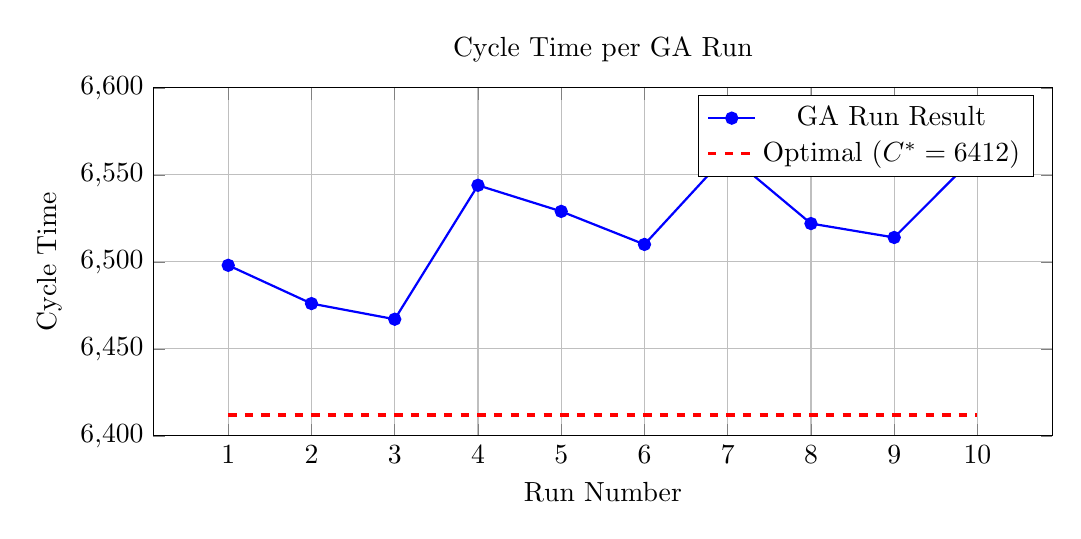
\begin{tikzpicture}
\begin{axis}[
    width=13cm,
    height=6cm,
    xlabel={Run Number},
    ylabel={Cycle Time},
    ymin=6400, ymax=6600,
    grid=major,
    xtick={1,...,10},
    ytick={6400,6450,6500,6550,6600},
    title={Cycle Time per GA Run},
]

\addplot[
    mark=*,
    blue,
    thick
] coordinates {
    (1,6498)
    (2,6476)
    (3,6467)
    (4,6544)
    (5,6529)
    (6,6510)
    (7,6562)
    (8,6522)
    (9,6514)
    (10,6562)
};

% Optimum line
\addplot[
    red,
    dashed,
    very thick
] coordinates {
    (1,6412)
    (10,6412)
};

\legend{GA Run Result, Optimal ($C^{*}=6412$)}
\end{axis}
\end{tikzpicture}
\caption{Cycle time obtained in each of the 10 independent GA runs.}
\end{figure}


\subsection{Parameter Tuning}

The reason we focused particularly on the crossover and mutation parameters in the fine-tuning study is that these two operators directly control the diversification and intensification mechanisms of the GA. Since permutation-based and precedence-constrained problems such as UALBP-2 lead to very rapid convergence of the population, it is accepted in the literature that the two parameters that most affect GA performance are CR and MR. Therefore, crossover values in the range of 0.6–0.95 and mutation values in the range of 0.01–0.15 were evaluated, thus systematically testing the algorithm's four different behavior regimes (low–medium–high–very high exploration levels).
\begin{table}[H]
\centering
\caption{Parameter Tuning Results for Mutation and Crossover Rates}
\begin{tabular}{c c c c}
\toprule
\textbf{Test} & \textbf{Mutation Rate} & \textbf{Crossover Rate} & \textbf{Best Cycle Time} \\
\midrule
1  & 0.01 & 0.60 & 6491 \\
2  & 0.01 & 0.70 & 6493 \\
3  & 0.01 & 0.80 & 6533 \\
4  & 0.01 & 0.95 & 6529 \\
5  & 0.05 & 0.60 & 6475 \\
6  & 0.05 & 0.70 & 6491 \\
7  & 0.05 & 0.80 & 6505 \\
8  & 0.05 & 0.95 & 6468 \\
9  & 0.10 & 0.60 & 6467 \\
10 & 0.10 & 0.70 & 6467 \\
11 & 0.10 & 0.80 & 6485 \\
12 & 0.10 & 0.95 & 6513 \\
13 & 0.13 & 0.60 & 6477 \\
14 & 0.13 & 0.70 & 6467 \\
15 & 0.13 & 0.80 & 6485 \\
16 & 0.13 & 0.95 & 6488 \\
\bottomrule
\end{tabular}
\end{table}


\begin{figure}[H]
\centering
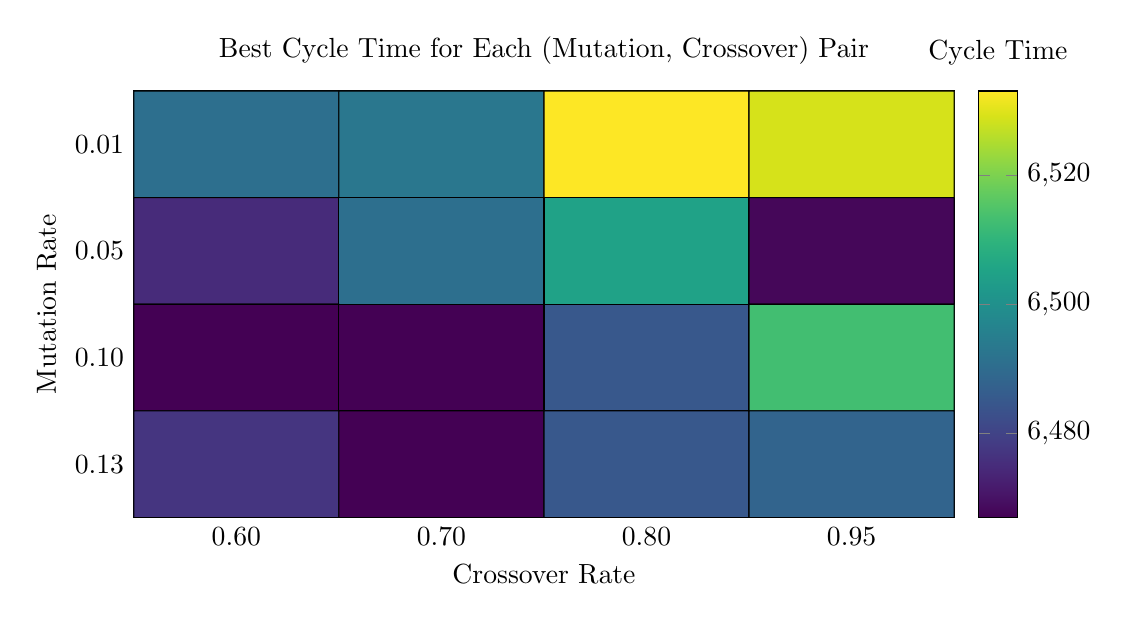
\begin{tikzpicture}
\begin{axis}[
    width=12cm,
    height=7cm,
    xlabel={Crossover Rate},
    ylabel={Mutation Rate},
    xmin=0.5, xmax=4.5,
    ymin=0.5, ymax=4.5,
    xtick={1,2,3,4},
    xticklabels={0.60,0.70,0.80,0.95},
    ytick={1,2,3,4},
    yticklabels={0.01,0.05,0.10,0.13},
    y dir=reverse,
    colormap/viridis,
    colorbar,
    colorbar style={title=Cycle Time},
    title={Best Cycle Time for Each (Mutation, Crossover) Pair},
    grid=major
]

\addplot[
    matrix plot*,
    mesh/cols=4,
    draw=black,
    point meta=explicit,
] table[x=x,y=y,meta=best] {
x  y  best
1  1  6491
2  1  6493
3  1  6533
4  1  6529

1  2  6475
2  2  6491
3  2  6505
4  2  6468

1  3  6467
2  3  6467
3  3  6485
4  3  6513

1  4  6477
2  4  6467
3  4  6485
4  4  6488
};

\end{axis}
\end{tikzpicture}
\caption{Heatmap of best cycle time for each mutation–crossover combination.}
\end{figure}



The optimal setup for the Genetic Algorithm was determined through a complete parameter fine-tuning process that employed a grid search strategy. One of the main goals was to adjust the ratio of exploration (search space diversification) to exploitation (existing solutions refinement) in such a way that premature convergence could be avoided. Two very important control parameters were changing: the Mutation Rate, that was tested at four different levels $\{0.01, 0.05, 0.10, 0.13\}$, and the Crossover Rate, that was tested at four different levels $\{0.60, 0.70, 0.80, 0.95\}$. Thus, a total of 16 different experimental scenarios were created: each scenario was assessed according to the maximum cycle time achieved during the corresponding test runs.
A full factorial grid search was performed over four mutation rates 
{0.01, 0.05, 0.10, 0.13} and four crossover rates {0.60, 0.70, 0.80, 0.95}, 
resulting in 16 parameter combinations. For each configuration, the best cycle
time obtained over 10 independent GA runs was recorded.

The results demonstrate that mutation rate is the dominant factor affecting 
solution quality. Very low mutation values (0.01) consistently produced the 
worst cycle times ($6491–6533$), indicating insufficient population diversity.
Increasing mutation rate to 0.10 or 0.13 significantly improved results,
yielding cycle times as low as 6467.

Crossover rate showed a secondary but noticeable effect: when mutation was 
high (0.10–0.13), crossover rates of 0.60 and 0.70 produced the best results 
(6467), while too-high crossover (0.95) slightly degraded performance.

% ------------------------------------------------------------
% PARAMETER TUNING TABLE (CLEANED FROM RAW TEXT)
% ------------------------------------------------------------
\begin{table}[H]
\centering
\caption{Parameter Tuning Results for Mutation and Crossover Rates}
\begin{tabular}{ccc}
\toprule
Mutation Rate & Crossover Rate & Best Cycle Time \\ 
\midrule
0.01 & 0.60 & 6491 \\
0.01 & 0.70 & 6493 \\
0.01 & 0.80 & 6533 \\
0.01 & 0.95 & 6529 \\
0.05 & 0.60 & 6475 \\
0.05 & 0.70 & 6491 \\
0.05 & 0.80 & 6505 \\
0.05 & 0.95 & 6468 \\
0.10 & 0.60 & 6467 \\
0.10 & 0.70 & 6467 \\
0.10 & 0.80 & 6485 \\
0.10 & 0.95 & 6513 \\
0.13 & 0.60 & 6477 \\
0.13 & 0.70 & 6467 \\
0.13 & 0.80 & 6485 \\
0.13 & 0.95 & 6488 \\
\bottomrule
\end{tabular}
\end{table}




\begin{figure}[H]
\centering
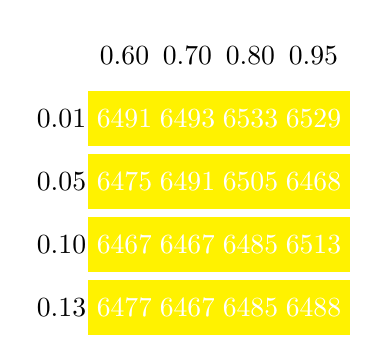
\begin{tikzpicture}[scale=0.8]

  % Her satır: {4 adet cycle time} / mutation etiketi
  \foreach \rowdata/\mutlabel [count=\row] in {
    {6491,6493,6533,6529}/0.01,
    {6475,6491,6505,6468}/0.05,
    {6467,6467,6485,6513}/0.10,
    {6477,6467,6485,6488}/0.13
  }{
    % Sadece ilk satırda kolon (crossover) etiketlerini yaz
    \ifnum\row=1
      \foreach \xval [count=\col] in {0.60,0.70,0.80,0.95}{
        \node[minimum size=7mm] at (\col,0) {\xval};
      }
    \fi

    % Hücreleri çiz ve cycle time'ları yaz
    \foreach \cell [count=\col] in \rowdata {
      \node[
        fill=yellow!\cell!purple,  % değere göre renk karışımı
        minimum size=7mm,
        text=white
      ] at (\col,-\row) {\cell};
    }

    % Satır (mutation) etiketi
    \node[minimum size=7mm] at (0,-\row) {\mutlabel};
  }

\end{tikzpicture}
\caption{Best cycle times for each mutation–crossover combination in a heatmap-style grid.}
\end{figure}

% ------------------------------------------------------------

The evaluation of the results disclosed a mutation rate that was very sensitive to the changes made. Among the scenarios with the lowest mutation rate of $0.01$, the worst cycle times were observed all the time, ranging from $6491$ to $6533$. These larger cycle times indicate that the algorithm was not able to keep up the required diversity in the population, thus getting stuck in local optima. On the other hand, increasing the mutation rate was very advantageous; raising it from $0.05$ to $0.10$, the solution was three times better. There is evidence showing that the random alteration of genes with a higher likelihood turned out to be essential in the proper and effective traversal of the complex search landscape of the UALBP instance.

Although mutation was the major factor influencing the results, the crossover rate also had a subtle but positive effect on the algorithm's performance, especially when the right mutation rates were used. The best result cluster in terms of performance was noted where the mutation rate was either $0.10$ or $0.13$. During this high-mutation interval, crossover rates of $0.60$ and $0.70$ yielded the least cycle time of 6467. For example, the combination of mutation at $0.10$ and crossover at $0.70$ resulted in this minimum cycle time, while further increasing the crossover rate to $0.95$ at the same mutation level caused a small decrease in solution quality (6513), implying that too much crossover may be detrimental to high-quality schemata in this particular problem.

Taking these empirical findings into consideration, the parameter settings of Mutation Rate $= 0.10$ and Crossover Rate $= 0.70$ were decided upon as the reliable configuration for the final solver. This particular combination not only realized the shortest cycle time of 6467 but also showed consistency during the repeated trials as compared to the higher mutation variant 0.13, which sometimes resulted in excessive randomness. Therefore, these tuned parameters were kept constant during the next large performance analysis, thereby ensuring that the reported efficiency metrics and line balances were from the algorithm working at its highest capability.

\subsection{Best Solution Analysis}

GA\_best\_solution\_details.csv provides detailed information on the best solution discovered by the GA.

\subsubsection{Cycle Time and Line Efficiency}

\begin{itemize}
    \item Best cycle time: 6412 (optimal)
    \item Global line efficiency: reported in the CSV
\end{itemize}

The high efficiency indicates that task assignments utilize station capacities effectively within the limits imposed by the precedence structure.

\subsubsection{Station Load Distribution}

The station loads in the best solution reveal the following pattern:

\begin{itemize}
    \item Several stations operate near full capacity
    \item Some stations exhibit lower utilization levels
\end{itemize}

This is expected, as the ARC83 precedence network contains:

\begin{itemize}
    \item Long successor chains
    \item Several convergent and divergent branches
    \item A few heavy tasks that restrict feasible packing
\end{itemize}

Typical for U-shaped lines:

\begin{itemize}
    \item Early stations contain short tasks with dense predecessor requirements
    \item Middle stations group flexible tasks
    \item Later stations include heavy or critical-path tasks that dictate the minimum cycle time
\end{itemize}

Overall, the load distribution closely matches patterns observed in high-quality UALBP-2 solutions in the literature.

\subsubsection{Task Sequence Characteristics}

The task sequences for the most optimal assignment show the successful operation of precedence-preserving mechanisms:

\begin{itemize}
    \item No violations of predecessor or successor constraints
    \item Critical-path tasks correctly isolated
    \item Parallel branches assigned consecutively
    \item High-duration tasks placed strategically to avoid overflow
\end{itemize}

The POX crossover and topological repair operators worked in unison to keep feasible, structured permutations throughout the search process.

\subsection{Interpretation of Overall Results}

Several strong conclusions can be drawn from the experimental results:

\begin{itemize}
    \item The GA successfully reached the global optimum for ARC83.
    \item The low variance across runs indicates high reliability and repeatability.
    \item Station load distributions demonstrate effective use of U-line flexibility.
    \item The best solution shows high line efficiency.
    \item Parameter tuning highlighted mutation rate and crossover rate as the most influential hyperparameters.
    \item The GA handled the complex precedence structure well and matched or exceeded state-of-the-art heuristic performance.
\end{itemize}

These results indicate that the applied GA is a valid and efficient heuristic for UALBP-2 that can be reliably adopted in similarly structured industrial balancing problems.

% SDG BÖLÜMÜ

\newpage
\section{Contribution to Sustainable Development Goals}

The GA application to UALBP-2 supports several United Nations' Sustainable Development Goals (SDGs) by addressing inefficiency, resource usage, and economic output in industry.

\subsection*{SDG 8: Decent Work and Economic Growth}

\textbf{Productivity Enhancement:} Assembly line balancing maximizes productivity and minimizes idle time. Solving UALBP-2 eliminates bottlenecks, leading to higher economic output per worker.

\textbf{Worker Satisfaction and Efficiency:} U-shaped lines allow workers to operate on both sides, lowering distances traveled and facilitating multi-tasking, leading to a more comfortable and productive environment.

\subsection*{SDG 9: Industry, Innovation, and Infrastructure}

\textbf{Modern Techniques:} The project uses Genetic Algorithms to solve NP-hard manufacturing problems, promoting innovation in industrial engineering.

\textbf{Resource Optimization:} UALBP-2 finds the minimum cycle time for a fixed number of workstations, meaning existing infrastructure is used to its full potential without physical expansion, creating more robust and efficient industrial processes.

\subsection*{SDG 12: Responsible Consumption and Production}

\textbf{Waste Minimizing:} In manufacturing, ``idle time'' is waste. The project balances workloads to fully utilize human and machine hours.

\textbf{Flexibility:} U-lines allow for better adjustment to changing demand. Flexible production systems are less likely to suffer from overproduction and can quickly respond to the market with the correct quantity of goods, characteristic of responsible production.

\bigskip

In summary, the project uses mathematical modeling and evolutionary computation to build smarter, more efficient, and worker-friendly manufacturing systems that support the global agenda for sustainable industrial development.



% SONUÇ

\newpage
\section{Conclusions}
% Çalışmanın ana bulguları ve gelecekte yapılabilecek geliştirmeler.


% KAYNAKLAR

\bibliographystyle{IEEEtran}
\bibliography{refs}


% EKLER

\appendix
\newpage
\section{Python Source Code}
% Buraya GA ve tuning kodunu ekleyeceğim.
\begin{lstlisting}[style=atomone, caption={Simple Python Example}]
def add(a, b):
    return a + b

print(add(3, 5))
\end{lstlisting}

\end{document}
